\section{Word to word models} \label{sec: text based models and architecture}
The harder challenge lies in processing natural languages. For this purpose two different approaches, namely the \nameref{subsubsec: onehot approach} and the \nameref{subsubsec: word vector approach} were examined. The ambitious goal was to learn or get a sense of the grammatical structure of the text. In practice, this means that after feeding \eg an adjective into the Neural Network, it should propose words or word classes which follow this word.
%Since the book is written in german, \texttt{Nouns} and \texttt{Adjectives} are obvious candidates for a successor but since it's free word order it is not possible to rely on these word classes since german has a variable word order\TODO{Vllt. ausführlicher schildern und/oder Referenz im Todo-Kommentar der tex-Datei hinzufügen}.
%% TODO https://en.wikipedia.org/wiki/V2_word_order#Examples_of_verb_second_(V2)
In the following paragraphs an schematic outline of the model will be given \ie few data was involved to achieve more reasonable diagrams. The full book covers multiple thousands of states, leading to a sparse squared matrix in this dimension. Thus, depicting matrices no longer makes sense.

To be able to evaluate the results, a ground truth distribution was calculated for gaining a qualitative and quantitative measure (\figref{\ref{fig: text model gt}}). The data set is labeled on the axes. There is also a \gls{mds} plot next to it because on large scale models ($ > 500 $ words) it is impossible to get visual feedback just by inspecting the matrix plot. The hope is that clusters of the same color appear as in \secreff{sec: first model and architecture MR}, because meta word pairs, for example \texttt{Noun → Verb} \eg \texttt{Alice → goes} and \texttt{wood → breaks}, should share some features and be mapped close to each other. Furthermore, similarities are to some extent also visible by looking at the \gls{mds}.

Having a reference now, the model was set up for training. In \figref{\ref{fig: text model sr}} is an emblematic transition matrix illustrated. Whereas in \secreff{sec: first model and architecture MR}, it was easy to recognize the rules in the \gls{sr}, this will no longer be possible due to the sheer amount of states. Hence, the cluster plot is more important to gain visual intuition for the results.
%
\begin{figure}
	\centering
		\subcaptionbox{Examplary ground truth distribution of a tiny data set.}{
		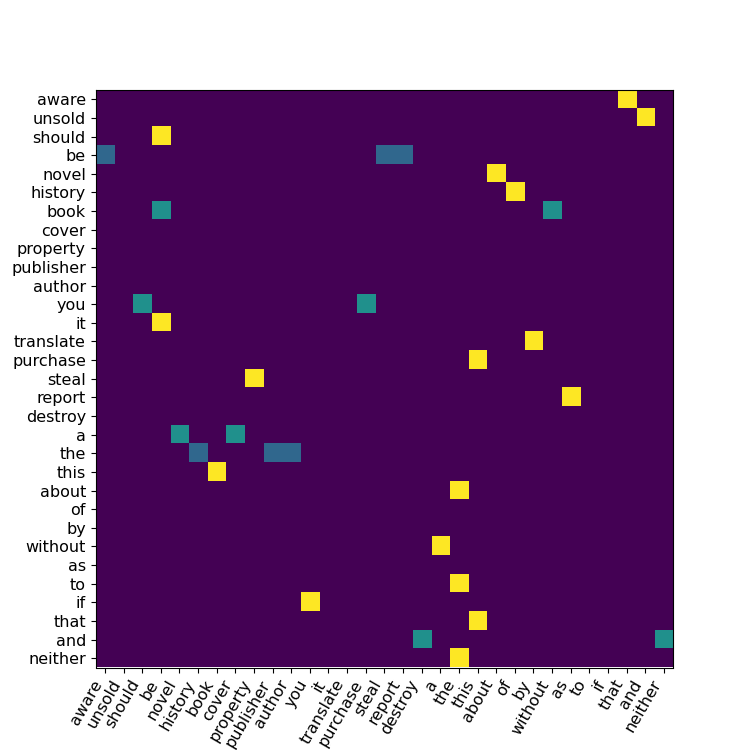
\includegraphics[height=\twocolpicheight]{Bilder/chapter4/BspW2W/plots/OHE_OHE_500E_100BS_1L_1C_5P_30T_J/J_5pages_30T_words.png}
	}
		\hfill
		\subcaptionbox{Corresponding \gls{mds} plot of the ground truth in (a).}{
			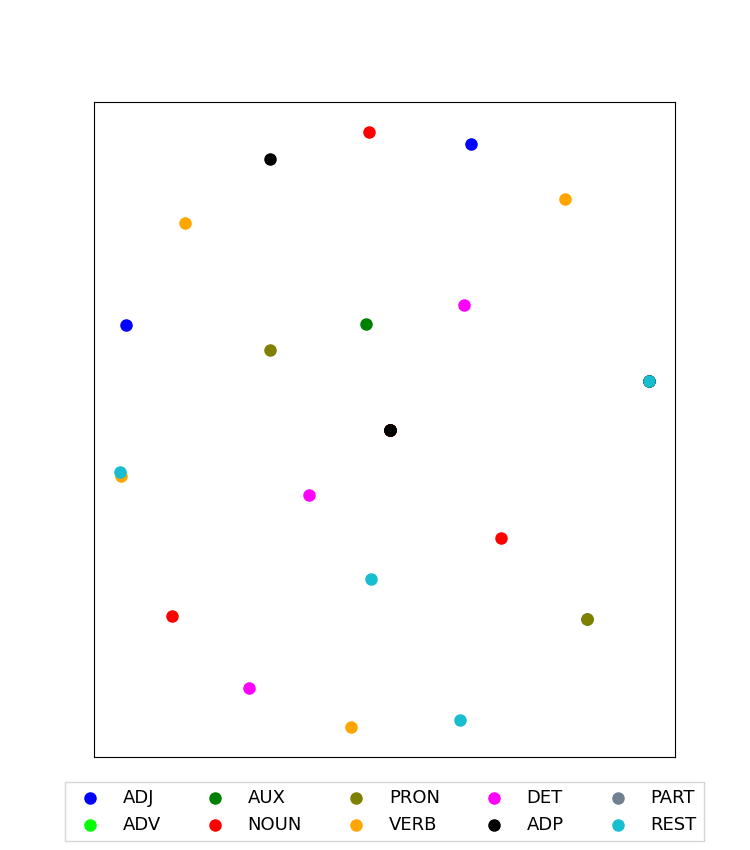
\includegraphics[height=\twocolpicheight]{Bilder/chapter4/BspW2W/plots/OHE_OHE_500E_100BS_1L_1C_5P_30T_J/MDS_J_5pages_30T_words.png}
		}
	\caption{For illustrative purposes only a tiny data set \ie few words of the book were processed to calculate the ground truth distribution.}
	\label{fig: text model gt}
\end{figure}
%
\begin{figure}
	\centering
		\subcaptionbox{Learned \srmat{} of model using \onehot{s} during training.}{
			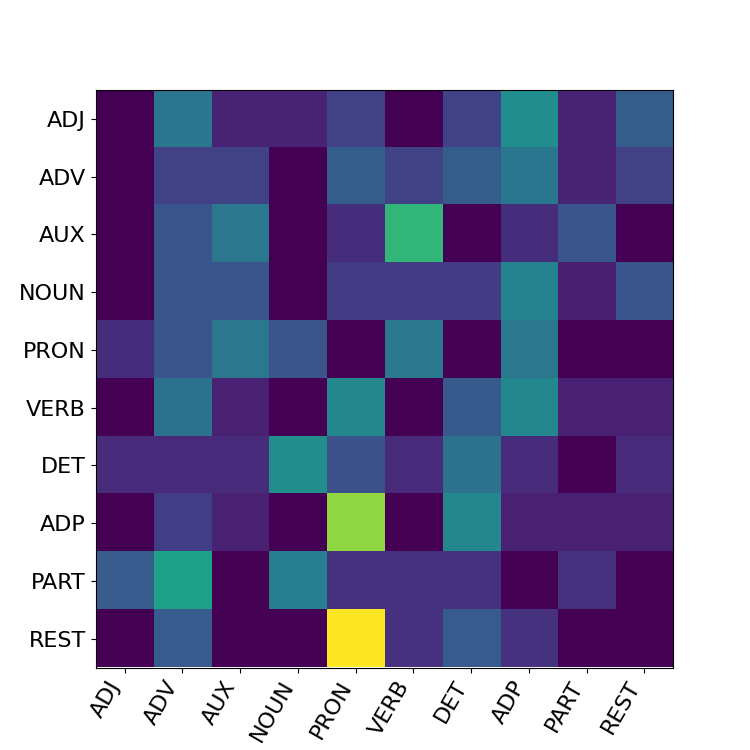
\includegraphics[height=\twocolpicheight]{chapter4/BspW2W/plots/OHE_OHE_500E_100BS_1L_1C_5P_30T_J/Transition_Probability_Matrix;_t=1,_DF=0.5.png}
		}
		\hfill
		\subcaptionbox{\gls{mds} clustering of the Successor Representation in (a).}{
			\includegraphics[height=\twocolpicheight]{chapter4/BspW2W/plots/OHE_OHE_500E_100BS_1L_1C_5P_30T_J/MDS_of_Transition_Probability_Matrix;_t=1,_DF=0.5.png}
		}
	\caption{Transition probability matrix of a model using constructed rules by processing a book and \onehot{s} during training. Hence, the environment is no longer manufactured. Whereas the results of the models in \secreff{sec: first model and architecture MR} were fully described by the matrix plot, this will no longer be possible for large scale models because the matrix becomes to huge. As seen before, the \gls{mds} can occupy this role. If sufficient learning happened, clusters or similarities to the corresponding plot of the ground truth should be recognizable. (Though not when illustrating with the tiny data set.)}
	\label{fig: text model sr}
\end{figure}

% --------------------------------------

\subsection{Word to word models: Evaluating the results} \label{subsec: text model evaluating the results}
To achieve the best result, four configurations were tested and compared in \tabref{\ref{tab: text model versions and metrics}} by the metric introduced in \secreff{sec: metric}.
\begin{table}
	\centering
	\caption{Trained models with metric values regarding their corresponding ground truth. ``german'' and ``english'' refer to the book which provided the data set (s. \secreff{sec: data preparation}). The associated \gls{mds} plots for a qualitative feedback can be found in \figref{\ref{fig: text model gt de en mds}} and \figref{\ref{fig: text model cumulativ mds plots}} of \appref{ch: appendix text model}.}
	\begin{tabular}{ll}
		\toprule
		Version					& Metric \\
		\midrule
		german, \onehot{} 		& $ 0.08 $	\\% 0.08200
		german, word vector		& $ 0.74 $	\\% 0.74139
		english, \onehot{}		& $ 0.10 $	\\% 0.10021
		english, word vector	& $ 0.78 $	\\% 0.77522
		\bottomrule
	\end{tabular}
	\label{tab: text model versions and metrics}
\end{table}
Surprisingly, the german and english \onehot{} versions nearly don't differ. Not only regarding the model used to collect the data but in general. Due to the beforehand mentioned freer word order german incorporates, a better score for the english based models was expected.

It is obvious that the models using word vectors perform quite bad compared to the \onehot{} variants. The reason may be on one hand that language is a structural complex field and on the other that too many uncertainties are attached to word vectors. Learning is more difficult since $ 300 $ distinct values are involved, whereas a \onehot{} may be quite accurate if the learned version has its maximum near or at the index where the input vector is equal to $ 1 $. Also back-calculating the output to a word is a process of compromises because it is guaranteed that \spacy{} doesn't provide a word vector with the exact same components and it is necessary to limit on the $ n $ closest word vectors/words. The disappointing outcome of the word vector model is furthermore frustrating since it is more probable that the hippocampus doesn't process signals which are close to \onehot{s} (or an analogy of it) but rather multiple stimuli decoding different characteristics, thus more related to a word vector.

\paragraph{Additional configurations}
While searching for the best parameters, not just the four versions mentioned were examined. Most of the time was consumed by finding a promising setup. This is reflected by some parameters the framework provides (\eg \texttt{nmb\_hidden\_layers}, \secreff{ap: parameters}), which aren't necessary to reproduce the results presented in this work. A subset with illustrations and short documentation of all variants can be found in \appref{ch: additional configurations}.

% --------------------------------------

%%%\subsection{Additional configurations} \label{subsec: additional configurations}
%To draw a full picture, plenty of approaches which had the goal to improve the results will be mentioned in this chapter. Sadly, no one changed the outcome by any means. Facing this presented an enormous obstacle while researching. Some of them will be presented shortly in this chapter. In all cases it is obvious that these configurations were dead ends.
%
%The architectures included
%\begin{itemize}
%	\item different number of epochs from $ 100 $ to $ 50000 $
%	\item $ 2 $-hot-encoded vectors
%	\item an auto-encoder structure
%\end{itemize}
%
%% --------------------------------------
%
%\section{Multiple hidden layers} \label{subsubsec: multiple hidden layers}
%Different numbers of layers ranging from $ 1 $ to $ 100 $ were tested, some example results will be depicted. 
%\begin{figure}[H]
%	\centering
%	\subcaptionbox{\gls{sr} of a model using english and \onehot{s} with $ 40 $ hidden layers.}{
%		
\includegraphics[height=\twocolpicheight]{Bilder/chapter4/additional_configurations/OHE_OHE_4000E_100BS_40L_1C_200P_1500T_J/Transition_Probability_Matrix;_t=1,_DF=0.5.png}
%	}
%	\hfill
%	\subcaptionbox{\gls{mds} of the matrix in (a).}{
%		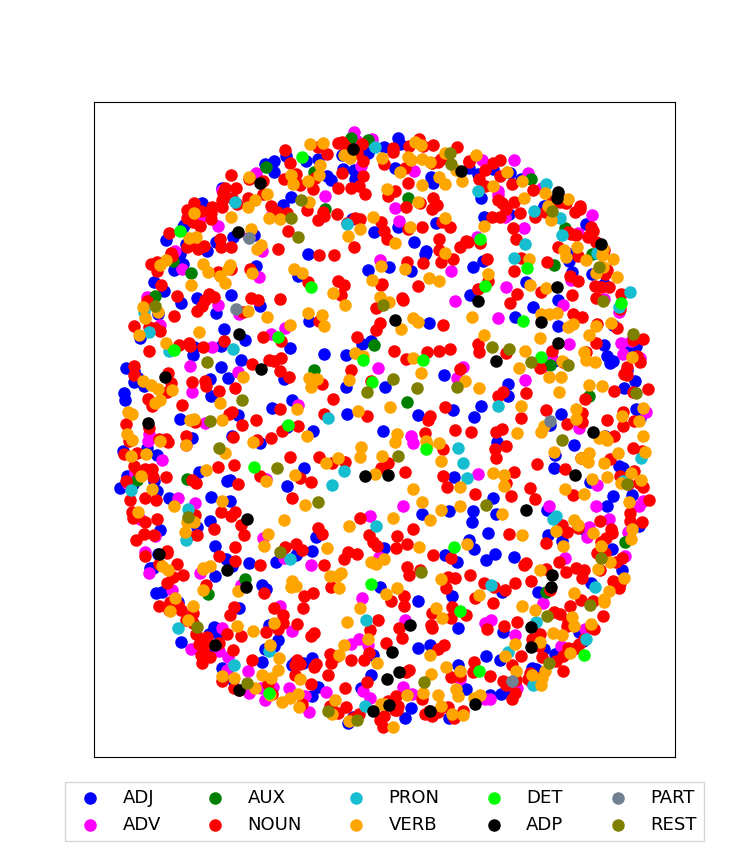
\includegraphics[height=\twocolpicheight]{Bilder/chapter4/additional_configurations/OHE_OHE_4000E_100BS_40L_1C_200P_1500T_J/MDS_of_Transition_Probability_Matrix;_t=1,_DF=0.5.png}
%	}
%	\caption{Although mentioned that transition probability matrices don't show anything if too many words are used, they can be used sometimes to detect failure. The reference, at least for the \gls{mds}, is illustrated in \figref{\ref{fig: w2w model gt en}}. The value of the metric is $ 0.50 $, the equivalent with one layer achieves $ 0.10 $ (s. \tabref{\ref{tab: text model versions and metrics}} to get a full list). This could imply that more layers hamper learning.}
%	\label{fig: text model en ohe 40L}
%\end{figure}
%%
%\begin{figure}[H]
%	\centering
%		\subcaptionbox{\gls{mds} of a model using english and \onehot{s} with $ 2 $ hidden layers.}{
%			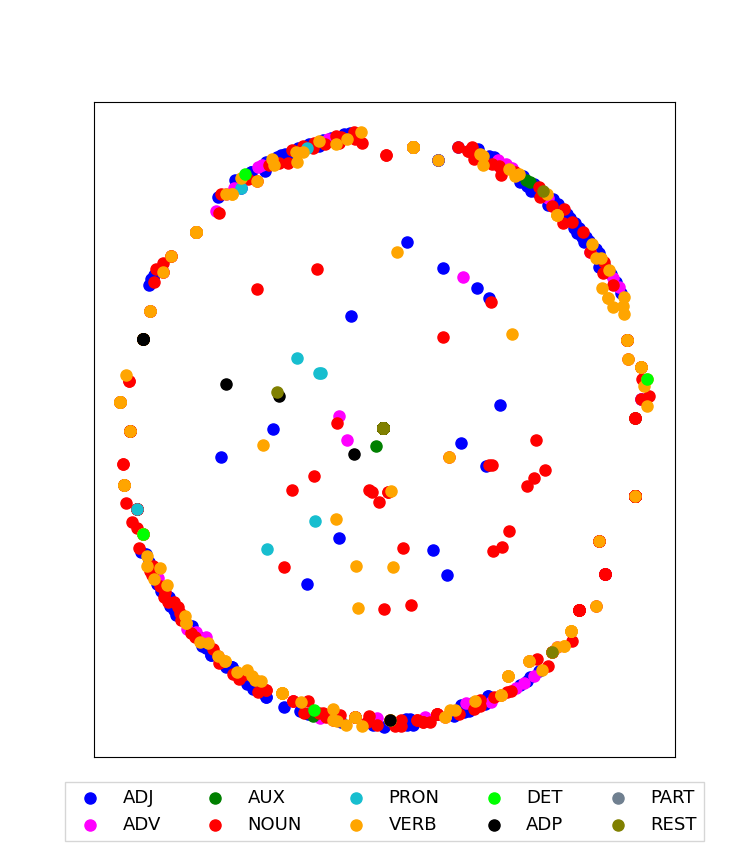
\includegraphics[height=\twocolpicheight]{Bilder/chapter4/additional_configurations/OHE_OHE_4000E_100BS_2L_1C_200P_1500T_J/MDS_of_Transition_Probability_Matrix;_t=1,_DF=0.5.png}
%		}
%		\hfill
%		\subcaptionbox{\gls{sr} of a model using english and \onehot{s} with $ 10 $ hidden layers.}{
%			
\includegraphics[height=\twocolpicheight]{Bilder/chapter4/additional_configurations/OHE_OHE_7000E_100BS_10L_1C_200P_1500T_J/Transition_Probability_Matrix;_t=1,_DF=0.5.png}
%		}
%	\caption{As mentioned before, more layers result in worse \glspl{sr}. Already one additional hidden layer lowers the metric. The model in (a) reaches $ 0.22 $, whereas with one hidden layer the value is $ 0.10 $. The network in (b) was configured with $ 10 $ hidden layers and the successor representation looks indistinguishable from one training with $ 40 $ (\figref{\ref{fig: text model en ohe 40L}}).}
%\end{figure}
%
%% --------------------------------------
%
%\section{Many epochs combined with multiple hidden layers}
%The example outputs stem from a model which trained with sixfold epochs and $ 40 $ hidden layers.
%\begin{figure}[H]
%	\centering
%		\subcaptionbox{English, \onehot{s}, $ 25,000 $ epochs and $ 40 $ layers.}{
%			
\includegraphics[height=\twocolpicheight]{Bilder/chapter4/additional_configurations/OHE_OHE_25000E_100BS_40L_1C_200P_1500T_J/Transition_Probability_Matrix;_t=1,_DF=0.5.png}
%		}
%		\hfill
%		\subcaptionbox{\gls{mds} of a model using english, word vectors, $ 25,000 $ epochs and $ 40 $ layers}{
%			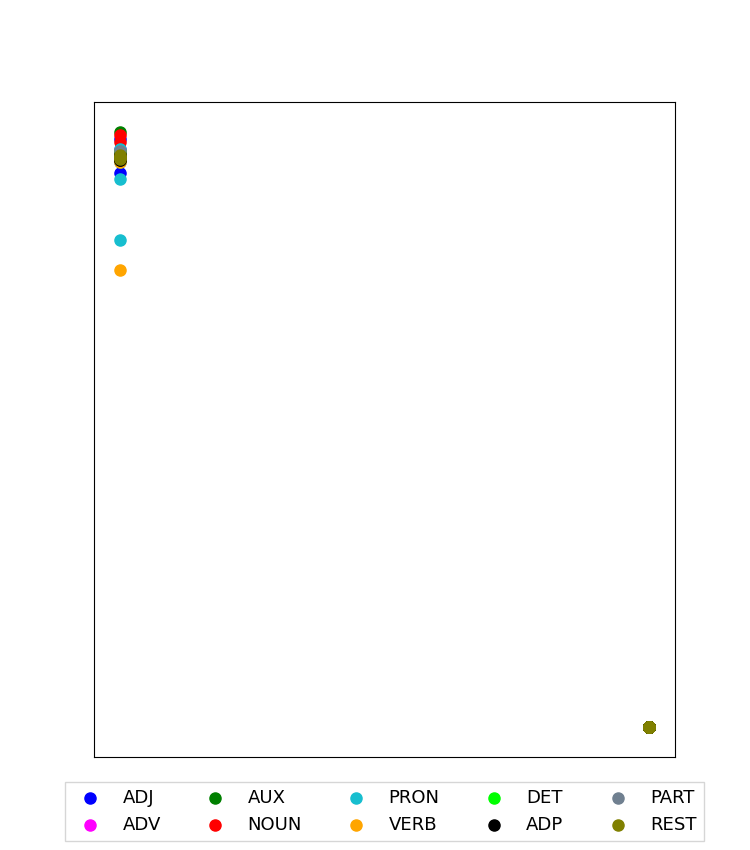
\includegraphics[height=\twocolpicheight]{Bilder/chapter4/additional_configurations/W2V_W2V_25000E_100BS_40L_1C_200P_1500T_J/MDS_of_Transition_Probability_Matrix;_t=1,_DF=0.5.png}
%		}
%	\caption{The only conclusion to draw from this plot of two different models is that additional epochs might lead to a full degeneration of the results if word vectors are used for training. The \onehot{} analogue shows no mismatch to them of \secreff{subsubsec: multiple hidden layers}.}
%\end{figure}
%
%% --------------------------------------
%
%\section{Using word vectors to learn an \onehot{}}
%This configuration is combination of two mainly used in the thesis. It uses word vectors as input and \onehot{s} as output \ie it uses heterogeneous structured training data.
%\begin{figure}[H]
%	\centering
%		\subcaptionbox{English, word vector to \onehot{} as \gls{mds}.}{
%			\includegraphics[width=\twocolpicwidth]{Bilder/chapter4/additional_configurations/W2V_OHE_5000E_100BS_1L_1C_200P_1500T_D/MDS_of_Transition_Probability_Matrix;_t=1,_DF=0.5.png}
%		}
%	\hfill
%		\subcaptionbox{German, ground truth \gls{mds} of word to word transitions.}{
%			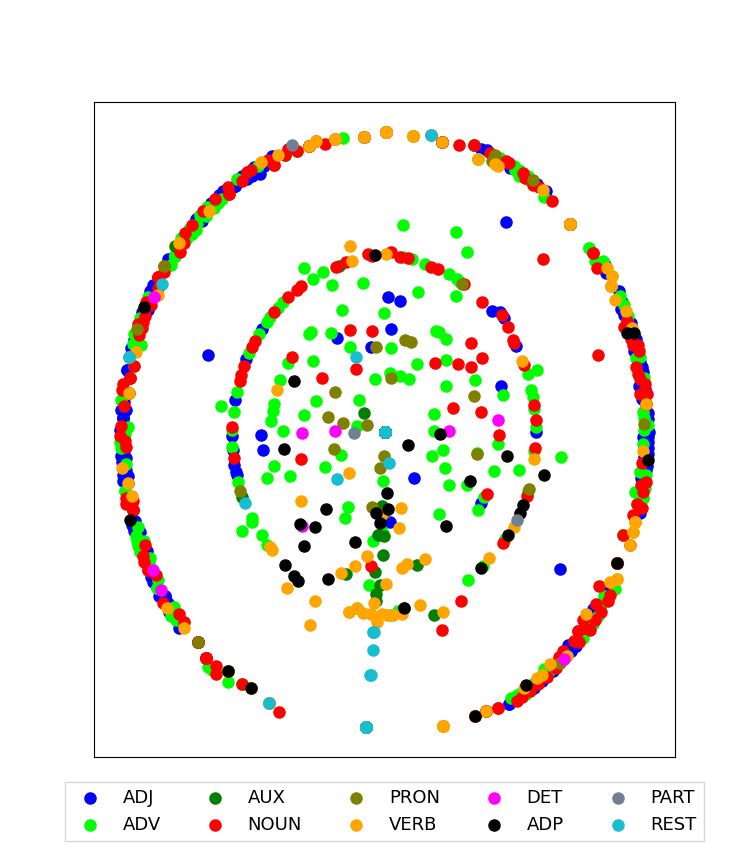
\includegraphics[width=\twocolpicwidth]{Bilder/chapter4/W2W/ground_truths/MDS_D_200pages_1500T_words.png}
%		}
%	\caption{\gls{mds} plot of a model using german training data and word vectors as input to learn a \onehot{}. The results lack characteristics to draw sensible conclusions from. Though it is possible to calculate the metric for the configuration: $ 0.47 $. By comparing with \tabref{\ref{tab: text model versions and metrics}}, it sits between its full \onehot{} and word vector relatives.}
%\end{figure}
%
%% --------------------------------------
%
%\section{Multiplying the training data} \label{subsubsec: multiplying training data}
%The goal of multiplying the training data \ie concatenating the training data $ n $ times with itself, was to have the opportunity to see the training data more often during one epoch.
%\begin{figure}[H]
%	\centering
%		\subcaptionbox{German, \onehot{s} with $ 5 $ concatenations.}{
%			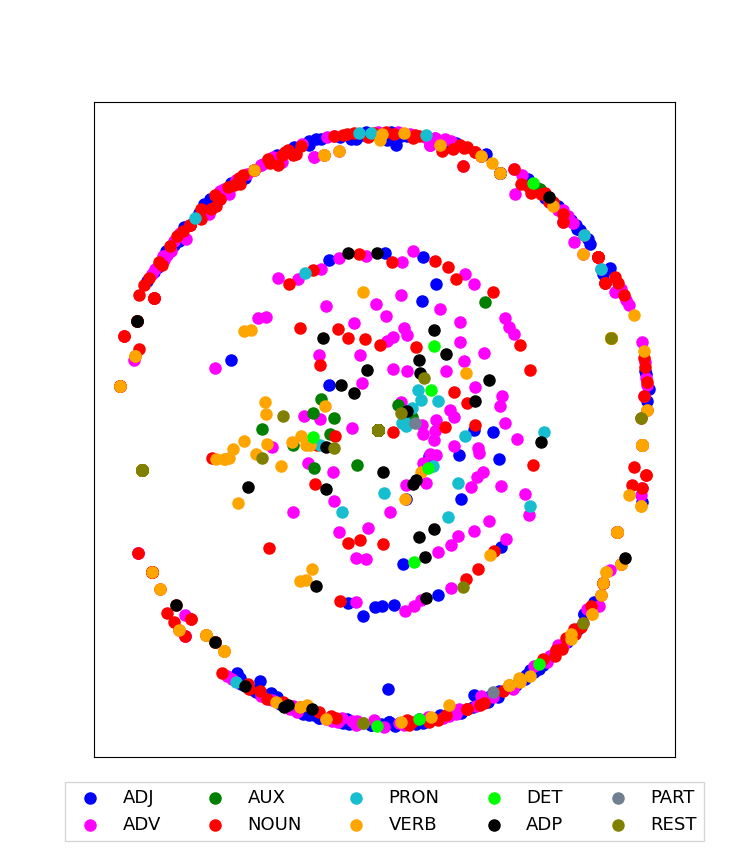
\includegraphics[width=\twocolpicwidth]{Bilder/chapter4/additional_configurations/OHE_OHE_5000E_100BS_1L_5C_200P_1500T_D/MDS_of_Transition_Probability_Matrix;_t=1,_DF=0.5.png}
%		}
%		\hfill
%		\subcaptionbox{German, word vectors with $ 5 $ concatenations.}{
%			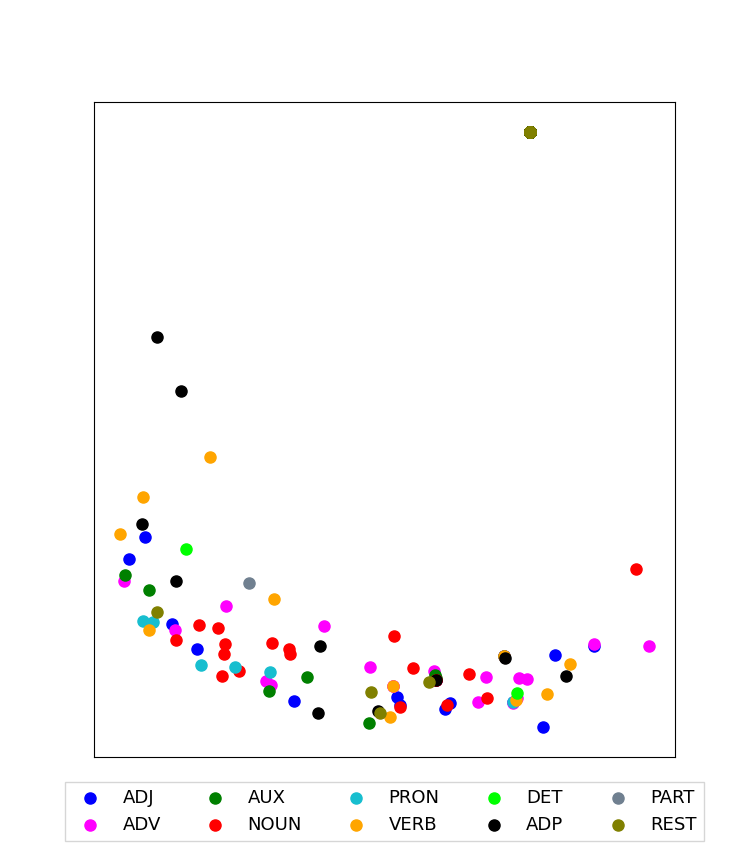
\includegraphics[width=\twocolpicwidth]{Bilder/chapter4/additional_configurations/W2V_W2V_5000E_100BS_1L_5C_200P_1500T_D/MDS_of_Transition_Probability_Matrix;_t=1,_DF=0.5.png}
%		}
%	\caption{Concatenating the training data $ 5 $ times with itself doesn't change outcomes (compare \figref{\ref{fig: text model cumulativ mds plots}}). This impression is fortified by the metrics both models achieve: $ 0.14 $ for \onehot{s} and $ 0.72 $ with word vectors ($ 0.08 $ and $ 0.74 $ without respectively, \tabref{\ref{tab: text model versions and metrics}}).}
%\end{figure}
%
%% --------------------------------------
%
%\section{Calculating high time steps}
%One idea was to calculate high time steps of the \gls{sr} hoping the irregularities even out in distant future.
%\begin{figure}[H]
%	\centering
%		\subcaptionbox{\gls{mds} of a \gls{sr} with $ t = 20 $. German and \onehot{s} were used during training.}{
%			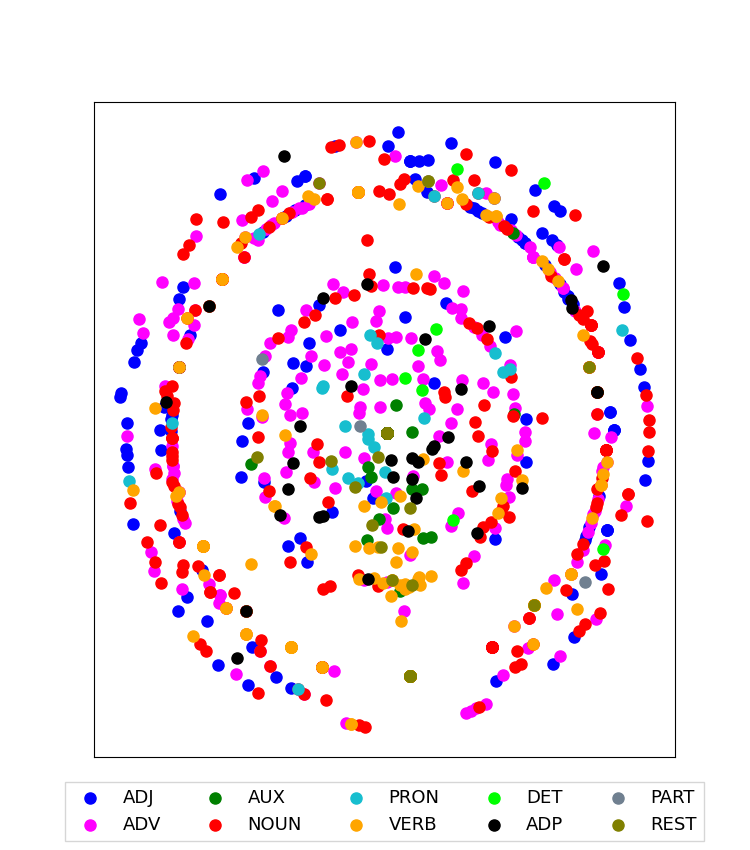
\includegraphics[width=\twocolpicwidth]{Bilder/chapter4/additional_configurations/hohes_t/OHE_OHE_5000E_100BS_1L_1C_200P_1500T_D/MDS_of_SR,_t=20,_DF=0.5.png}
%		}
%		\hfill
%		\subcaptionbox{\gls{mds} of a \gls{sr} with $ t = 50 $. German and \onehot{s} were used during training.}{
%			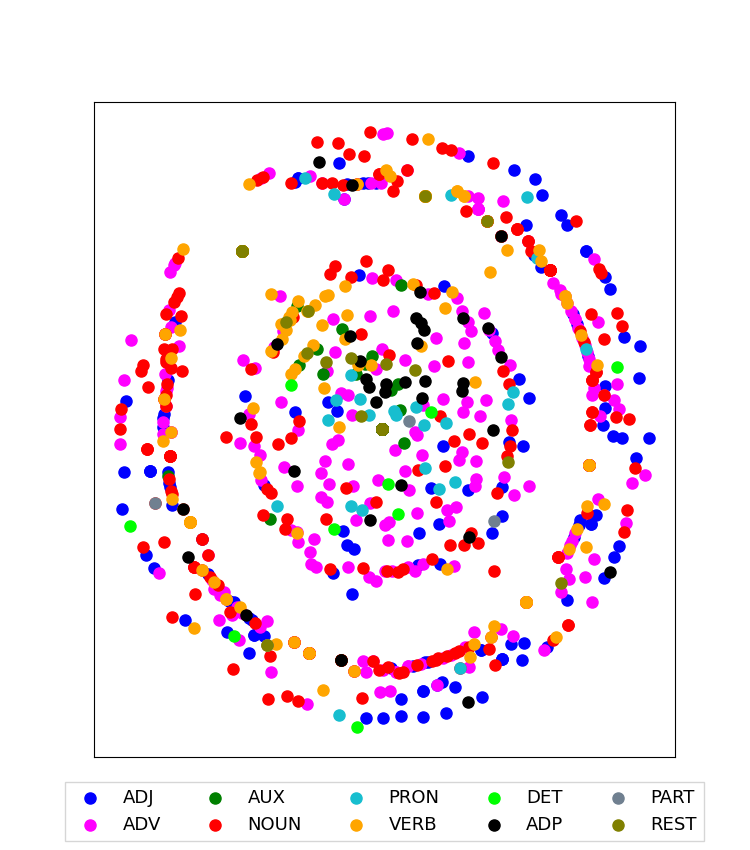
\includegraphics[width=\twocolpicwidth]{Bilder/chapter4/additional_configurations/hohes_t/OHE_OHE_5000E_100BS_1L_1C_200P_1500T_D/MDS_of_SR,_t=50,_DF=0.5.png}
%		}
%	\caption{High times also don't bring progress since no evident structure is recognizable within the plots. A comparison with the ground truth wouldn't bring additional insights too because the underlying matrices can't be interpreted as transition probability matrices.}
%	\label{fig: high time steps ohe}
%\end{figure}
%%
%\begin{figure}[H]
%	\centering
%		\subcaptionbox{\gls{mds} of a \gls{sr} with $ t = 20 $. German and word vectors were used during training.}{
%			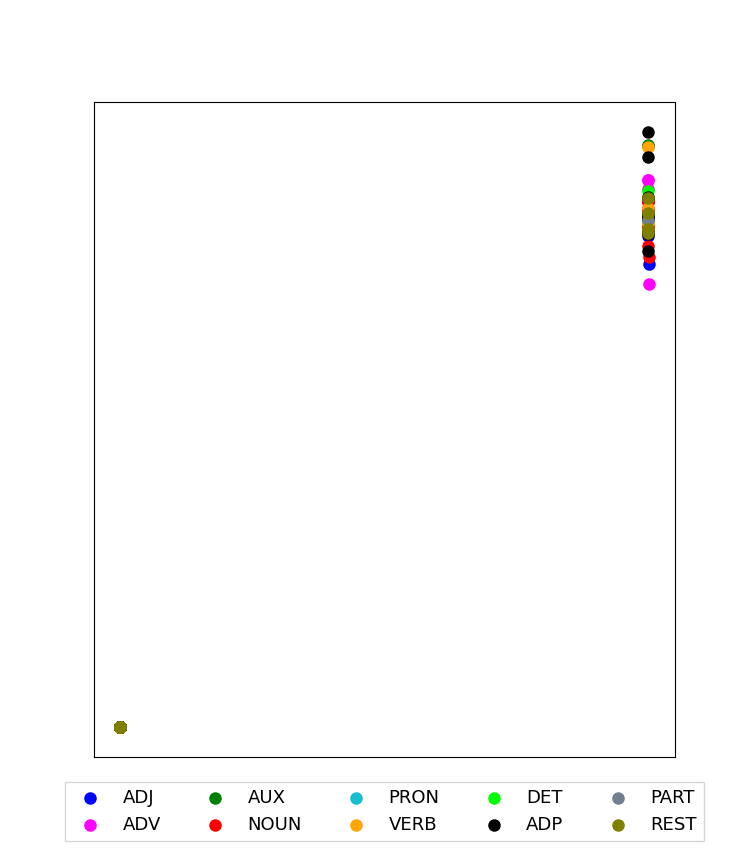
\includegraphics[width=\twocolpicwidth]{Bilder/chapter4/additional_configurations/hohes_t/W2V_W2V_5000E_100BS_1L_1C_200P_1500T_D/MDS_of_SR,_t=20,_DF=0.5.png}
%		}
%		\hfill
%		\subcaptionbox{\gls{mds} of a \gls{sr} with $ t = 50 $. German and word vectors were used during training.}{
%			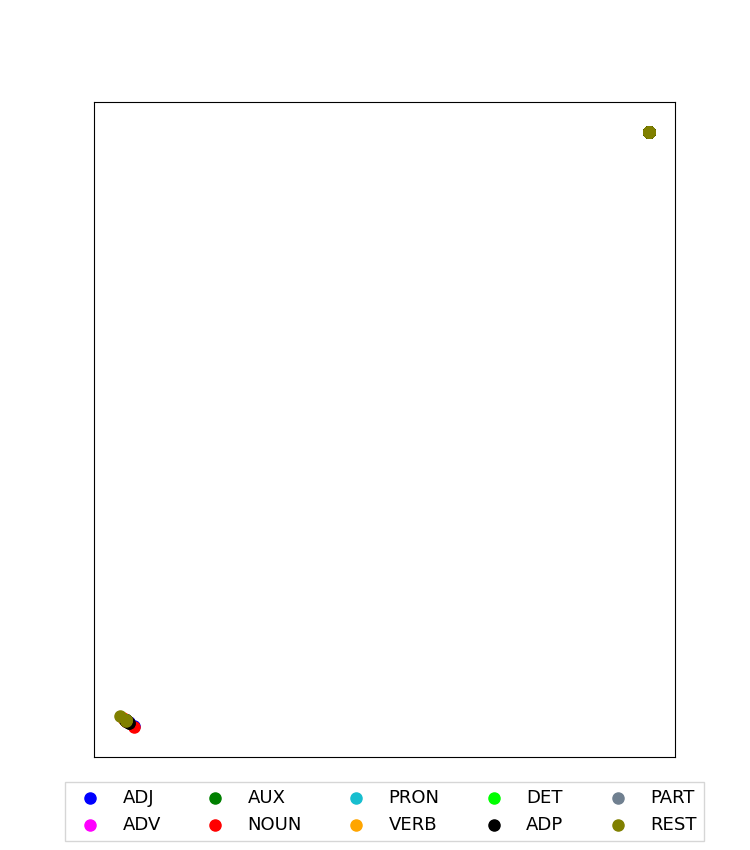
\includegraphics[width=\twocolpicwidth]{Bilder/chapter4/additional_configurations/hohes_t/W2V_W2V_5000E_100BS_1L_1C_200P_1500T_D/MDS_of_SR,_t=50,_DF=0.5.png}
%		}
%	\caption{As before in \figref{\ref{fig: high time steps ohe}} no structure is recognizable to do further research on. Results relying on word vectors again seem to be very labile and degenerate.}
%\end{figure}
%
%% --------------------------------------
%
%\section{Predict only the most frequent words}
%Similar to \secreff{subsubsec: multiplying training data}, the most frequent words of the text are seen more often by the network. Hence it might be able to learn these inputs better than ordinary ones.
%\begin{figure}[H]
%	\centering
%		\subcaptionbox{German with word vectors. \gls{mds} of the $ 40 $ most frequent words.}{
%			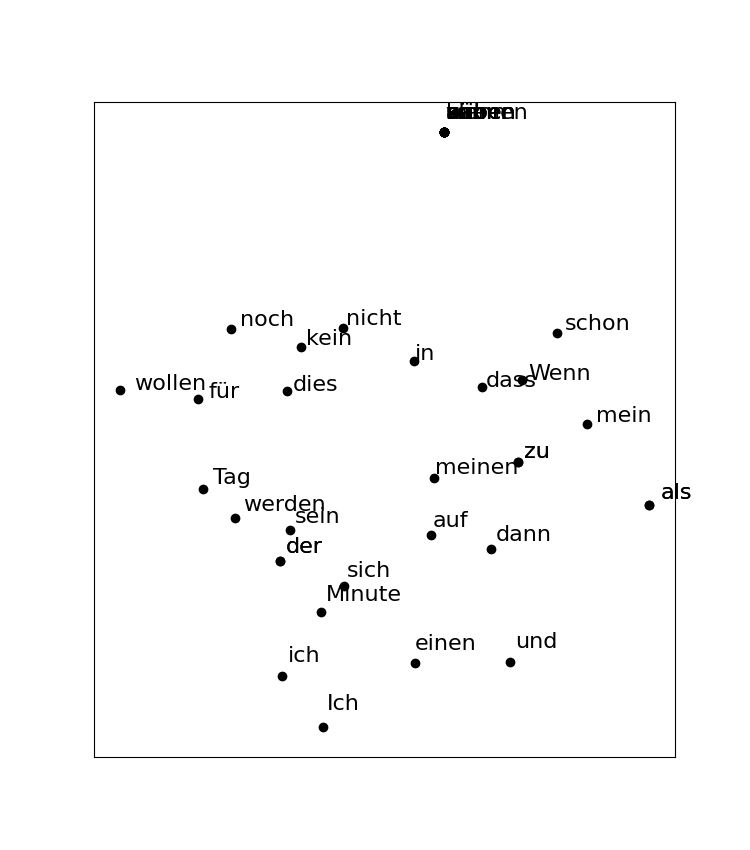
\includegraphics[width=\twocolpicwidth]{Bilder/chapter4/additional_configurations/MostFrequentWords_4000E_100BS_1L_1C_200P_1500T_D/MDS_of_Transition_Probability_Matrix;_t=1,_DF=0.5.png}
%		}
%		\hfill
%		\subcaptionbox{Same \gls{mds} plot as in (a) but annotated with \postag{s}instead of words.}{
%			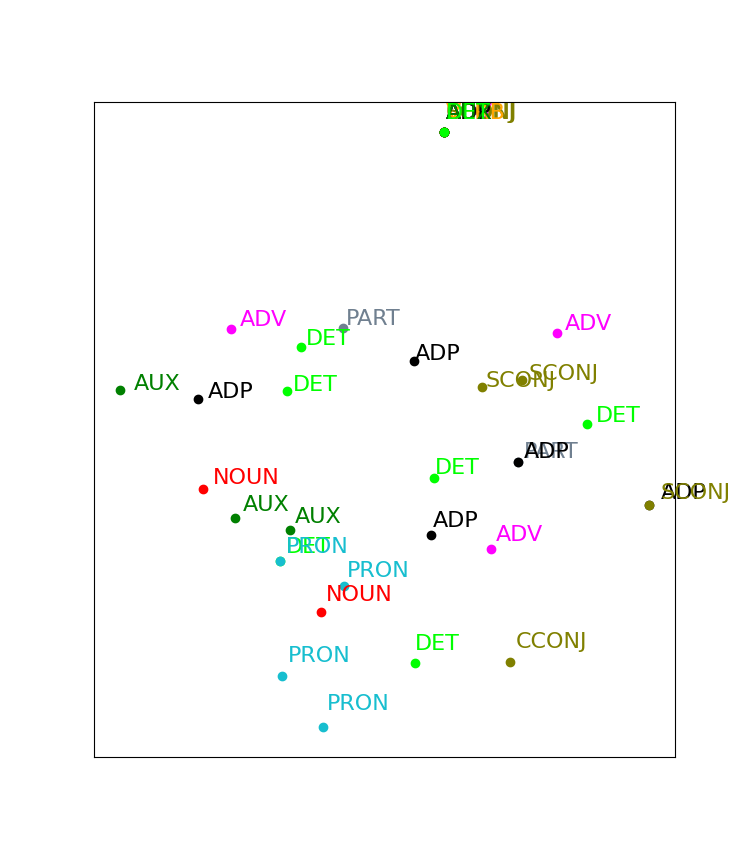
\includegraphics[width=\twocolpicwidth]{Bilder/chapter4/additional_configurations/MostFrequentWords_4000E_100BS_1L_1C_200P_1500T_D/ud_pos_tag_annotated.png}
%		}
%	\caption{The same model with german data set and word vectors as in \secreff{sec: text based models and architecture} was trained. Predictions were limited to the $ 40 $ most frequent words. For a better overview the second plot was labeled with the corresponding \postag{s}.}
%\end{figure}


%The ambitions goal of detecting grammatical rules by using encoded words as \onehot{} or word vector wasn't achieved by solely evaluating the plain word models.
